\documentclass[12pt,a4paper]{report}
\usepackage[utf8]{inputenc}
\usepackage[english]{babel}
\usepackage{graphicx}
\usepackage[left=2cm,right=2cm,top=2cm,bottom=2cm]{geometry}
\usepackage[T1]{fontenc}
\usepackage{amsmath}
\usepackage{amsfonts}
\usepackage{amssymb}
\usepackage{graphics}
\usepackage{epsfig}
\usepackage{listings}
\usepackage{enumerate}
\usepackage{lastpage}
\usepackage{setspace}
\usepackage{hyperref}
\usepackage[hang]{caption}
\usepackage{titling}
\usepackage{float}
\usepackage{listings}
\usepackage{color}
\definecolor{mygreen}{rgb}{0,0.6,0}
\definecolor{mygray}{rgb}{0.5,0.5,0.5}
\definecolor{mymauve}{rgb}{0.58,0,0.82}
\lstset{ 
  backgroundcolor=\color{white},   % choose the background color; you must add \usepackage{color} or \usepackage{xcolor}; should come as last argument
  basicstyle=\footnotesize,        % the size of the fonts that are used for the code
  breakatwhitespace=false,         % sets if automatic breaks should only happen at whitespace
  breaklines=true,                 % sets automatic line breaking
  captionpos=b,                    % sets the caption-position to bottom
  commentstyle=\color{mygreen},    % comment style
  deletekeywords={...},            % if you want to delete keywords from the given language
  escapeinside={\%*}{*)},          % if you want to add LaTeX within your code
  extendedchars=true,              % lets you use non-ASCII characters; for 8-bits encodings only, does not work with UTF-8
  firstnumber=1000,                % start line enumeration with line 1000
  frame=single,	                   % adds a frame around the code
  keepspaces=true,                 % keeps spaces in text, useful for keeping indentation of code (possibly needs columns=flexible)
  keywordstyle=\color{blue},       % keyword style
  language=Octave,                 % the language of the code
  morekeywords={*,...},            % if you want to add more keywords to the set
  numbers=left,                    % where to put the line-numbers; possible values are (none, left, right)
  numbersep=5pt,                   % how far the line-numbers are from the code
  numberstyle=\tiny\color{mygray}, % the style that is used for the line-numbers
  rulecolor=\color{black},         % if not set, the frame-color may be changed on line-breaks within not-black text (e.g. comments (green here))
  showspaces=false,                % show spaces everywhere adding particular underscores; it overrides 'showstringspaces'
  showstringspaces=false,          % underline spaces within strings only
  showtabs=false,                  % show tabs within strings adding particular underscores
  stepnumber=2,                    % the step between two line-numbers. If it's 1, each line will be numbered
  stringstyle=\color{mymauve},     % string literal style
  tabsize=2,	                   % sets default tabsize to 2 spaces
  title=\lstname                   % show the filename of files included with \lstinputlisting; also try caption instead of title
}
% drawing mode if necessary
%\usepackage{tikz}
%\usepackage{circuitikz}
\singlespacing
% \onehalfspacing
\hypersetup
{
  	colorlinks,
  	citecolor=black,
 	linkcolor=black,
  	urlcolor=black
}
\title{Project Laboratory} 
\author{Levente Dudas PhD}
\newcommand{\doctype}{Project Laboratory Report} 
\newcommand{\doctitle}{ARDF Receiver 80 m}

\begin{document}
\begin{titlepage}

\begin{figure}
\centering

\includegraphics[width=100mm,keepaspectratio]{bme.pdf}
\end{figure}

\centering
\textbf{Budapesti Műszaki és Gazdaságtudományi Egyetem}\\
\textbf{Villamosmérnöki és Informatikai Kar}\\
\textbf{Szélessávú Hírközlés és Villamosságtan Tanszék}\\
\vspace{5mm}

\includegraphics[width=40mm,keepaspectratio]{hvt_logo_only_fixed_vector_inverted.png}  \\
\vspace{50mm}
\Huge
\dokumentumcim\\
\vspace{60mm}
\Large
\thetitle \\
\vspace{12mm}
\Large
\textbf{\theauthor}\\
\vspace{12mm}
\the\year


\end{titlepage}
\tableofcontents
\chapter*{Abstract}

This document is ggg a \LaTeX -based template for the BSc/MSc thesis of students at the Electrical Engineering and Informatics Faculty of Budapest University of Technology and Economics. The usage of this template is optional. It has been tested with the TeXLive TEX implementation, and it requires the PDF-LaTeX compiler.
\chapter{The 2 halves of the Project Laboratory semester}

The semester is divided into two parts.

\section{The first half}

From the first to the 7 th. week: common circuit realization, measurement and documentation in V1 502.

We will use: soldering stations, soldering irons, tin, cutter, tweezer, electrical components of the circuit, PCB, oscilloscope, probes, digital multimeters.

During the first 7 weeks, there will be at least 6 laboratory presentations / introductions.

\section{The second half}

8-14 week: there are differential tasks under laboratory supervision in different laboratories (as you selected in the 7 th. week): Tab. \ref{tab:lab}.

\begin{table}[hb]
        \footnotesize
        \centering
        \caption{Laboratories and Lab. Leaders}
        \begin{tabular}{ | l | l |}
        \hline
        Name of Lab. & Lab. Leader\\
        \hline
 		Antennas and EMC & Lajos Nagy PhD \\
 		DOCS & János Bitó PhD \\
 		EMF & József Pavo PhD\\
 		Microwave Remote Sensing Lab. & Rudolf Seller PhD\\
 		NES & András Reichardt \\
 		Space Technology & László Csurgai-Horváth PhD\\
        \hline
        \end{tabular}
        \label{tab:lab}
\end{table}

\section{15th week}

After the semester, before the exam period, oral session will be held in the same time as ProjLab (friday, 8-12h).

These oral presentations have to be presented by every students based on the second half of the semester (what happened in the Labs, only the work): 5 min presentation, 2 min questions. Only \LaTeX pdf (beamer) allowed with static contents.

\section{Result}

3 \LaTeX compiled pdfs are necessary for the final mark calculation:

\begin{enumerate}
\item Measurement report of the realized circuit (first half, common work, 5-10 effective pages) - 33 \%.
\item Report of the second half of the semester, containing the work you had been done (5-10 eff. pages) - 33 \%.
\item Oral presentaton of the second half of the semester (5 min = 5 effective slides) - 34 \%.
\end{enumerate}

The effective slides of the oral presentation can be counted without the title slide, the outline, the content, and the acknowledgement.

Do NOT use the string of "Thank you for your kind attention!" as last slide, instead of it, you can show pictures on the last slide, what you have done in the semester. The usage of the mentioned string means minus 1 mark.  

The comparision levels of the overall mark are: 40, 55, 70, 85 \%.

For instance:

\begin{enumerate}
\item Measurement report: 67 \%,
\item 2 nd. half report: 89 \%,
\item Oral presentation: 98 \%.
\end{enumerate}

The averaged percent is: $ round( \frac{67+89+98}{3} ) = 85 \% $, $ 70 < 85 \leq 85$ means 5 (excellent).

\section{Deadlines}

\begin{enumerate}
\item last day of the semester (14th week friday), 23:59:59 in e-mail,
\item wednesday of 15th week (two days before the oral session), 12:00:00 in e-mail,
\item thursday of 15th week (one day before the oral session), 12:00:00 in e-mail,
\end{enumerate}

all \LaTeX pdf as attachment to \url{dudas.levente@vik.bme.hu}.

\section{Equations}

If you want to use mathematical formulas, you can use this structure: \textit{equation}.

\begin{equation}
\centering
\ F ( \vartheta ) = \sum_{k=0}^{N-1} I_k \cdot e^{-jk \beta d cos \vartheta}
\label{eq:antsys}
\end{equation}

and after the formula \cite{diploma}, all variables must be defined as:

\begin{itemize}
\item where $ F ( \vartheta ) $ is the radiation pattern of the antenna system,
\item $ N $ is the number of the antenna elements,
\item $ I_k $ is the relative feeding current or voltages of the k th. of the antenna element,
\item $ k $ is the index of the antenna element,
\item $ \beta = \frac{2 \pi}{ \lambda } $ is the wave-number,
\item $ d $ is the equi-distance of the antenna elements in wavelength,
\item $ \vartheta $ is the direction of the incoming RF signal.
\end{itemize}

and of course, you can refenced this equation as: the radiation pattern of the antenna row can be calculated as Eq. \ref{eq:antsys}.
\chapter{Amateur Radio Direction Finder Receiver}

The circuit is designed in KiCad - \cite{kicad}

\begin{enumerate}
\item
The radio receiver:\\
	The main blocks:
	\begin{itemize}
	\item 9 turns from 210 cm CuZ copper wire as antenna,
	\item RF (radiofrequency) amplifier,
	\item RF band pass filter,
	\item BJT (bipolar junction transistor) based mixer,
	\item local oscillator,
	\item audio frequency low pass filter,
	\item audio amplifier.
	\end{itemize}
\item
The test transmitter:\\
	Collpitts type oscillator, where the quartz frequency is some 100 Hz different from the receiver local oscillator frequency, in order to make audio signal and it can be heard.
\end{enumerate}

\newpage
\section{Schematic}

The schematic diagram of the receiver is in Fig. \ref{fig:rokasch}.

\begin{figure}[H]
\centering
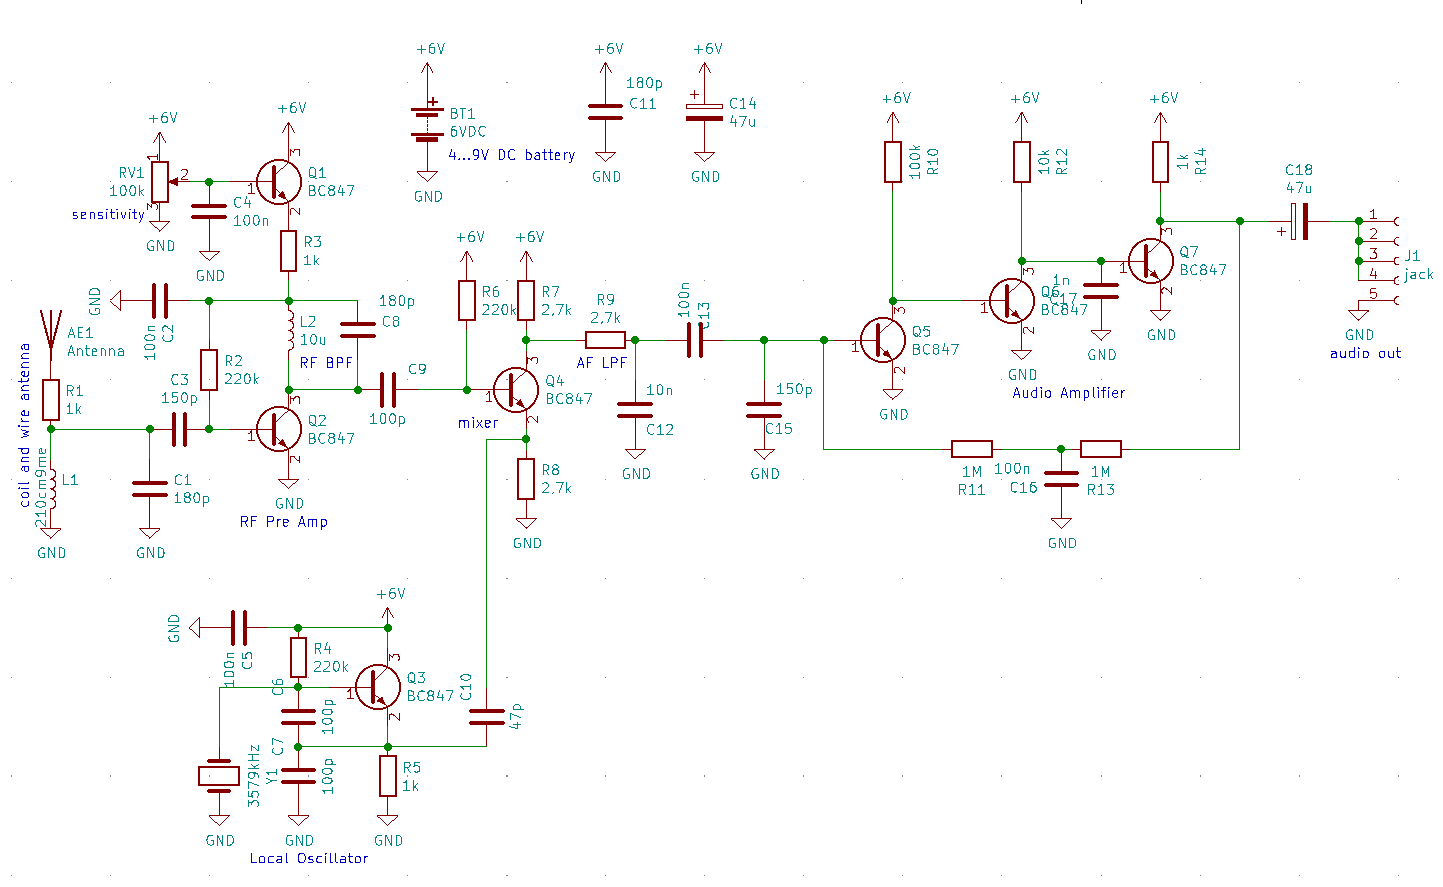
\includegraphics[width=1\textwidth]{../pic/sch.png}\\
\caption{Schematic}
\label{fig:rokasch}
\end{figure}

\newpage
\section{Printed Circuit Board}

The designed PCB can be seen in Fig. \ref{fig:rokanyhl}. There are THT and SMD type components.

\begin{figure}[H]
\centering
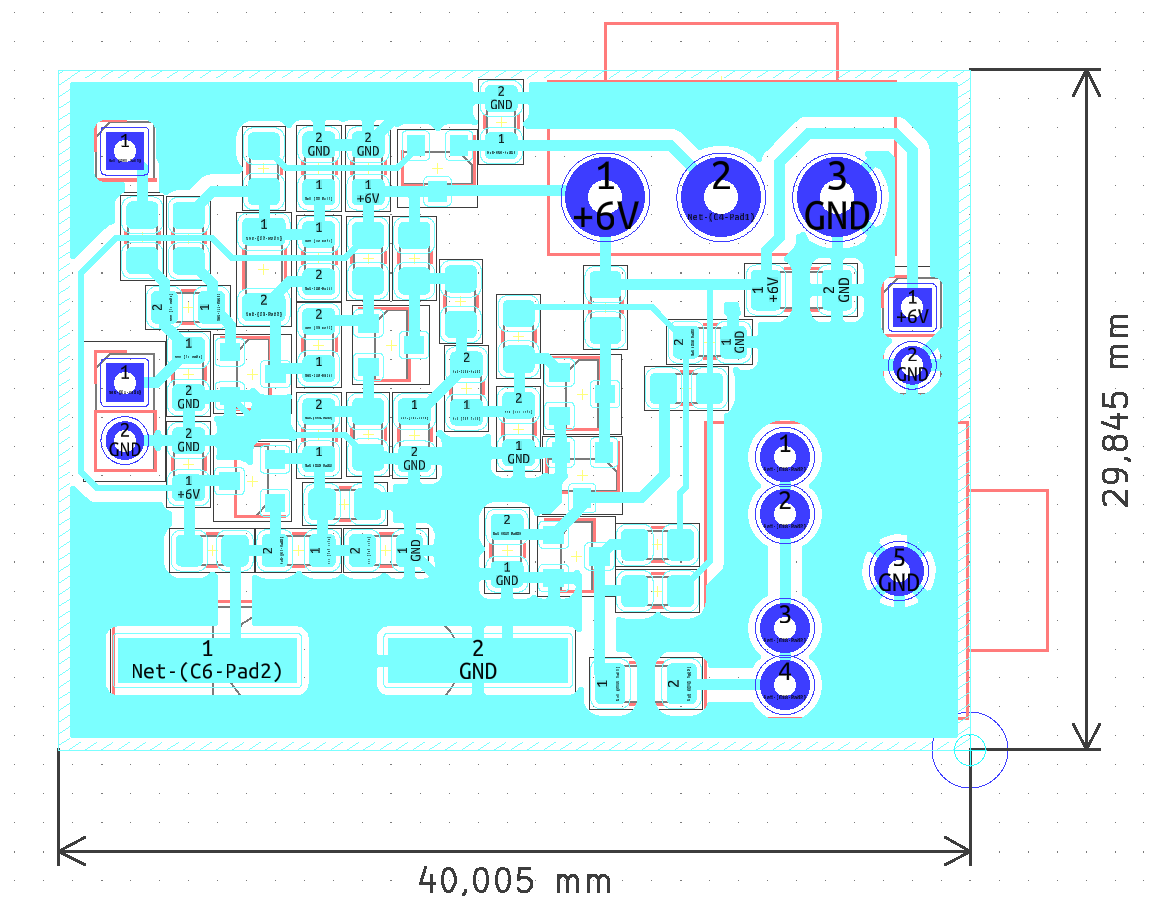
\includegraphics[width=1\textwidth]{../pic/pcb.png}
\caption{PCB}
\label{fig:rokanyhl}
\end{figure}

\newpage
\section{Component placement}

The components with its reference is in Fig. \ref{fig:rokault}.

\begin{figure}[H]
\centering
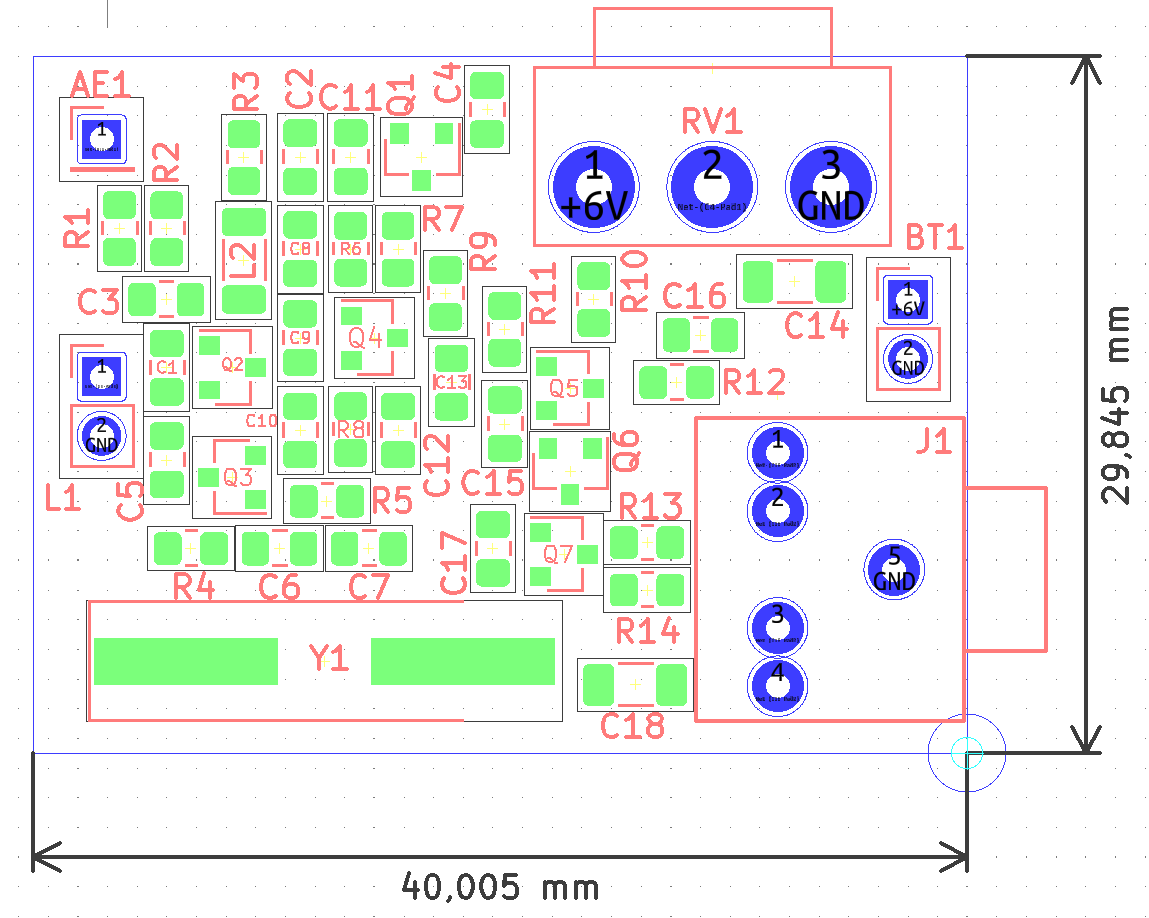
\includegraphics[width=1\textwidth]{../pic/pos.png}
\caption{Components Placement}
\label{fig:rokault}
\end{figure}

Placement order:

\begin{enumerate}
\item resistors,
\item capacitors,
\item inductors,
\item transistors,
\item connectors,
\item antenna.
\end{enumerate}

\newpage
\section{Measurement of the realized circuit}

The task is to measure the following parameters of the realized circuit and make test and measurement report based on the measurement results.

\begin{enumerate}
\item Bias DC voltages to the reference GND point on all pins of all semiconductors.
\item Voltage curve in time of the local oscillator output (emitter): peak-to-peak voltage, frequency, png from the scope.
\item Receiver audio (time domain) output signal on the AF output connector: variable resistor low, middle, high position: peak-to-peak voltage, frequency, curve. During this measurement, a single test transmitter will be run near to the receiver.
\end{enumerate}
\begin{thebibliography}{4}

\bibitem{hvthonlap} \url{http://hvt.bme.hu}

\bibitem{radiotechnika} Rádiótechnika évkönyve 2007, 172. oldaltól

\bibitem{diploma} Dudás Levente, \emph{Digitális nyalábformálású antenna (DBF)} diplomaterv, BME SzHVT, 2007

\bibitem{kicad} \url{http://kicad-pcb.org/}

\end{thebibliography}


\listoffigures
\listoftables
\chapter*{Appendix}

The chapter of appendix can contain: source codes, print-screens, figures, etc.

\section{while1 C source code}

The "while1" source code is here: \ref{app:while1}.

\lstinputlisting[language=C]{while1.c}
\label{app:while1}


\end{document}
